\section{Theoretische Grundlagen}
Der Lock-In-Verstärker ist ein Gerät, das ein periodisches Signal von einer bestimmten Frequenz empfangen und erkennen kann.
Dabei haben Störsignale einen nur geringen Einfluss auf die Messung des Signals.
% Vermutlich keine Subsection
\subsection{Funktionsweise}
Der Lock-In-Verstärker filtert das von außen kommende Signal $U_\text{sig}$ in zwei Schritten.
Der erste Schritt ist ein Bandpassfilter.
Dieser filtert alle Frequenzen heraus, die sehr weit von der Signalfrequenz $\omega$ entfernt sind.
Dazu muss der Bandpassfilter auf die Signalfrequenz eingestellt sein, damit er die richtigen Frequenzen filtern kann.
Im zweiten Schritt wird die Signalspannung $U_\text{sig}$ mit einer Referenzspannung $U_\text{ref}$ vermischt.
$U_\text{ref}$ ist eine Rechteckschwingung, die die gleiche Frequenz hat wie das ursprüngliche Signal $U_\text{sig}$.
Sie schwingt zwischen 1 und -1 und ist so normiert, dass sie den Betrag der Signalspannung nicht verändert.
Das Mischen lässt sich mathematisch durch eine Multiplikation $U_\text{sig} \cdot U_\text{ref}$ ausdrücken.
Durch einen Phasenschieber lässt sich $U_\text{ref}$ um die Phase $\Phi$ verschieben.
\begin{figure}
    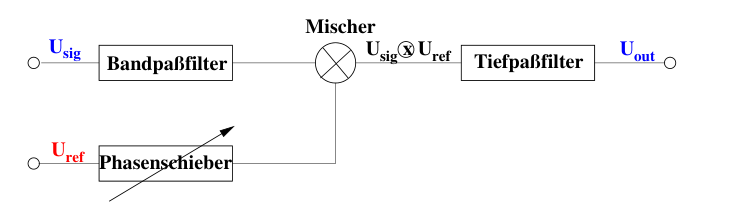
\includegraphics[width=\textwidth]{Abbildungen/Grundlegende_idee.png}
    \caption{Schematischer Aufbau des Lock-In-Verstärkers \cite[][]{man:v303}}
    \label{fig:grundlegende_Idee}
\end{figure}

In \cite[]{man:v303} wird dieser Prozess mit einem Sinusförmigen Beispielsignal durchgerechnet:
\begin{align}
    U_\text{sig} = U_{0} \sin(\omega t) 
\end{align}
Anschließend wird die Fourierreihe der Rechteckschwingung aufgestellt:
% 
\begin{align}
    U_\text{ref} = \frac{4}{\pi} \left(\sum_{k=0}^{\infty} \frac{1}{2k+1} \sin((2k+1)\omega t)\right)
\end{align}
Die Therme für $U_\text{ref}$ und $U_\text{sig}$ werden multipliziert
\begin{align}
    U_\text{sig} \cdot U_\text{ref} = 
    \frac{2}{\pi} U_0 \left(1 - \frac{2}{3} \cos(2 \omega t) - \frac{2}{15}\cos{4 \omega t} - \cdots \right) 
    \label{eq:Uref_Usig}
\end{align}
Die entstehende Schwingung enthält nun die geraden Oberwellen der Grundfrequenz \cite[vgl.][]{man:v303}.
Bei einem Phasenunterschied von $\Phi=0$ wirkt diese also wie ein Gleichrichter.
\begin{figure}
    \centering
    \includegraphics[width=0.3\textwidth]{Abbildungen/Signalverläufe.png}
    \caption{Signalverläufe bei einer sinusförmigen Signalspannung \cite{man:v303}}
    \label{fig:signalverlaeufe}
\end{figure}
Durch einen Tiefpassfilter, werden anschließend die schwingenden Anteile von \ref{eq:Uref_Usig} entfernt.
Übrig bleibt nur die erste Ordnung von \ref{eq:Uref_Usig}
\begin{align}
    U_\text{out} = \frac{2}{\pi} U_0
\end{align}
Wird das Referenzsignal um die Phase $\Phi$ zu $U_\text{sig}$ verschoben ergibt sich \cite[vgl.][]{man:v303}:
\begin{align}
    U_\text{out} = \frac{2}{\pi} U_0 \cos(\Phi)
    \label{eq:Uout_von_Phi}
\end{align}
% Was passiert wenn man eine Rechteckschwingung als Signal hat?
% Tiefpassfilter als Integrierglied
